\documentclass{article}
\usepackage{titling}
\usepackage{lipsum}
\usepackage{amsmath}
\usepackage{listings}
\usepackage{graphicx}
\usepackage{subcaption}
\usepackage{pgfplots}
\usepgfplotslibrary{statistics}



\begin{document}
\noindent
\begin{minipage}[t]{0.6\textwidth}
    \begin{flushleft}
        \LARGE\textbf{Math 343 - Homework 3} \\
        \vspace{6pt} % add 6pt of vertical space
        \hrule width 10cm
        \vspace{12pt}
        \large\textbf{Preston Duffield} \\
        \large Western Washington University \\
        % \today
        April 20, 2023
        \vspace{24pt}
    \end{flushleft}
\end{minipage}

\section*{Question 1}
\subsection*{a)}
\subsection*{b)}
\subsection*{c)}
\subsection*{d)}
\subsection*{e)}
\subsection*{f)}

\clearpage
\section*{Question 2}

\subsection*{a)}
$H_0$: All means are equal. \\
$H_a$: Not all means are equal. \\
\begin{figure}[h]
    \centering
    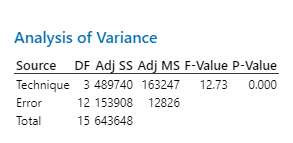
\includegraphics[width=0.5\textwidth]{./images/2_a.png}
    \caption{The output of the One-way ANOVA from Minitab.}
    \label{fig:2_a}
\end{figure}
Performing an F test at we can see that the P-value$ = 0.000 < \alpha = .05$, therefore we can conclude the following.
There is enough statistical evidence to support the hypothesis that not all means are equal.

\subsection*{b)}
\begin{figure}[h]
    \centering
    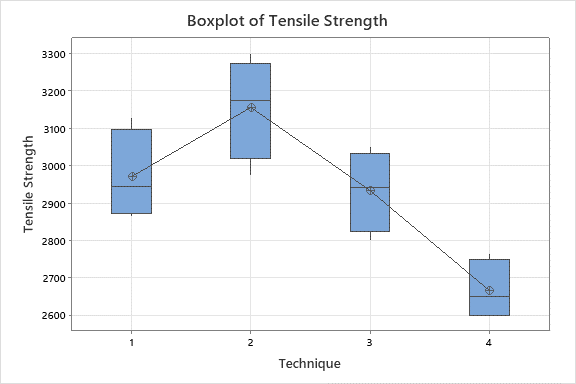
\includegraphics[width=1\textwidth]{./images/2_b.png}
    \caption{The Boxplot of tensile strength of the One-way ANOVA test from Minitab.}
    \label{fig:2_b}
\end{figure}
Judging by the boxplot alone, It would seem that the means are significantly different.
This is consistent with the above hypothesis test.
It looks as though the mean for treatment 1 and treatment 3 could be similar, in a pairwise comparison.
\subsection*{c)}
The results of the Fisher's LSD test can be summarized in the graphical results below.
Note that a line under the treatments indicate that they are not significantly different. \\
\vspace{12pt}
\\
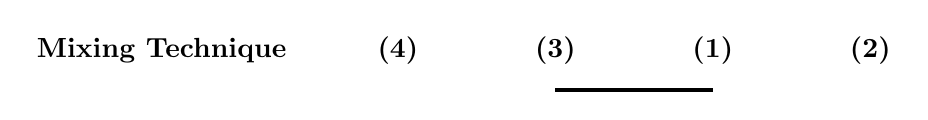
\begin{tikzpicture}[yscale=-1]
    % Define the positions of the labels
    \coordinate (labelPos) at (0, 0);
    \coordinate (4Pos) at (3, 0);
    \coordinate (3Pos) at (5, 0);
    \coordinate (1Pos) at (7, 0);
    \coordinate (2Pos) at (9, 0);

    % Draw the labels
    \node at (labelPos) {\textbf{Mixing Technique}}; % Treatment label
    \node at (4Pos) {\textbf{(4)}};
    \node at (3Pos) {\textbf{(3)}};
    \node at (1Pos) {\textbf{(1)}};
    \node at (2Pos) {\textbf{(2)}};

    % Draw the line
    \draw[ultra thick] ([yshift=0.5cm]3Pos) -- ([yshift=0.5cm]1Pos);
    % \draw[thick] ([yshift=1cm]1Pos) -- ([yshift=1cm]2Pos); % another theoretical line.
\end{tikzpicture}


\subsection*{d)}

\begin{figure}[h]
    \centering
    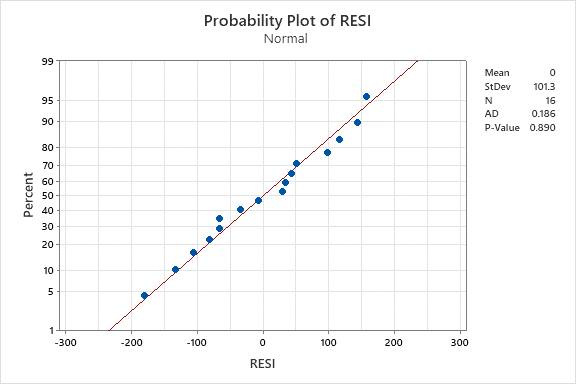
\includegraphics[width=1\textwidth]{./images/2_d.png}
    \caption{The normal probability plot of the residuals from Minitab.}
    \label{fig:2_d}
\end{figure}
\begin{flushleft}
$H_0$: The data are drawn from a normal disribution. \\
$H_a$: The data are not drawn from a normal disribution. \\
\end{flushleft}
Since the P-value is very large (0.890), we can conclude the following. 
The evidence of the data is consistent with the data being drawn from a normal disribution.

\subsection*{e)}
\begin{figure}[h]
    \centering
    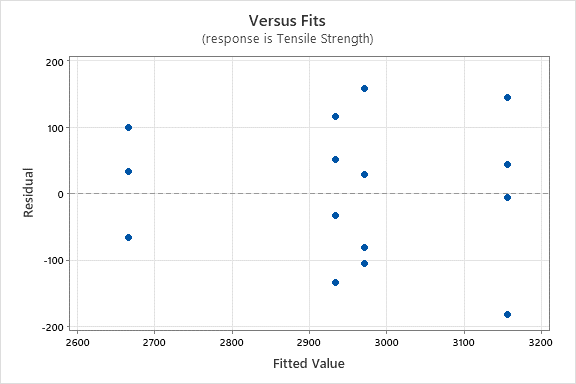
\includegraphics[width=1\textwidth]{./images/2_e.png}
    \caption{The residuals versus the predicted tensile strength from Minitab.}
    \label{fig:2_e}
\end{figure}
This graph indicates that there is not heteroskedasticity present,
that along with the conclusion that the data is drawn from
a normal distribution indicates that the model assumptions are verified
and the hypothesis test is valid.

\clearpage
\section*{Question 3}
\subsection*{a)}

\clearpage
\section*{Question 4}
\subsection*{a)}
\subsection*{b)}
\subsection*{c)}
\subsection*{d)}
\subsection*{e)}

\clearpage
\section*{Question 5}
\subsection*{a)}
\subsection*{b)}
\subsection*{c)}
\subsection*{d)}

\clearpage
\section*{Question 6}

\clearpage
\section*{Question 7}

\end{document}
